\hypertarget{part-1-design-1}{%
	\section{Part 1}\label{part-1-design-1}}

\centering


\hypertarget{description}{%
	\subsubsection{Description}\label{description}}

\begin{description}
	\item[Image:]
	\item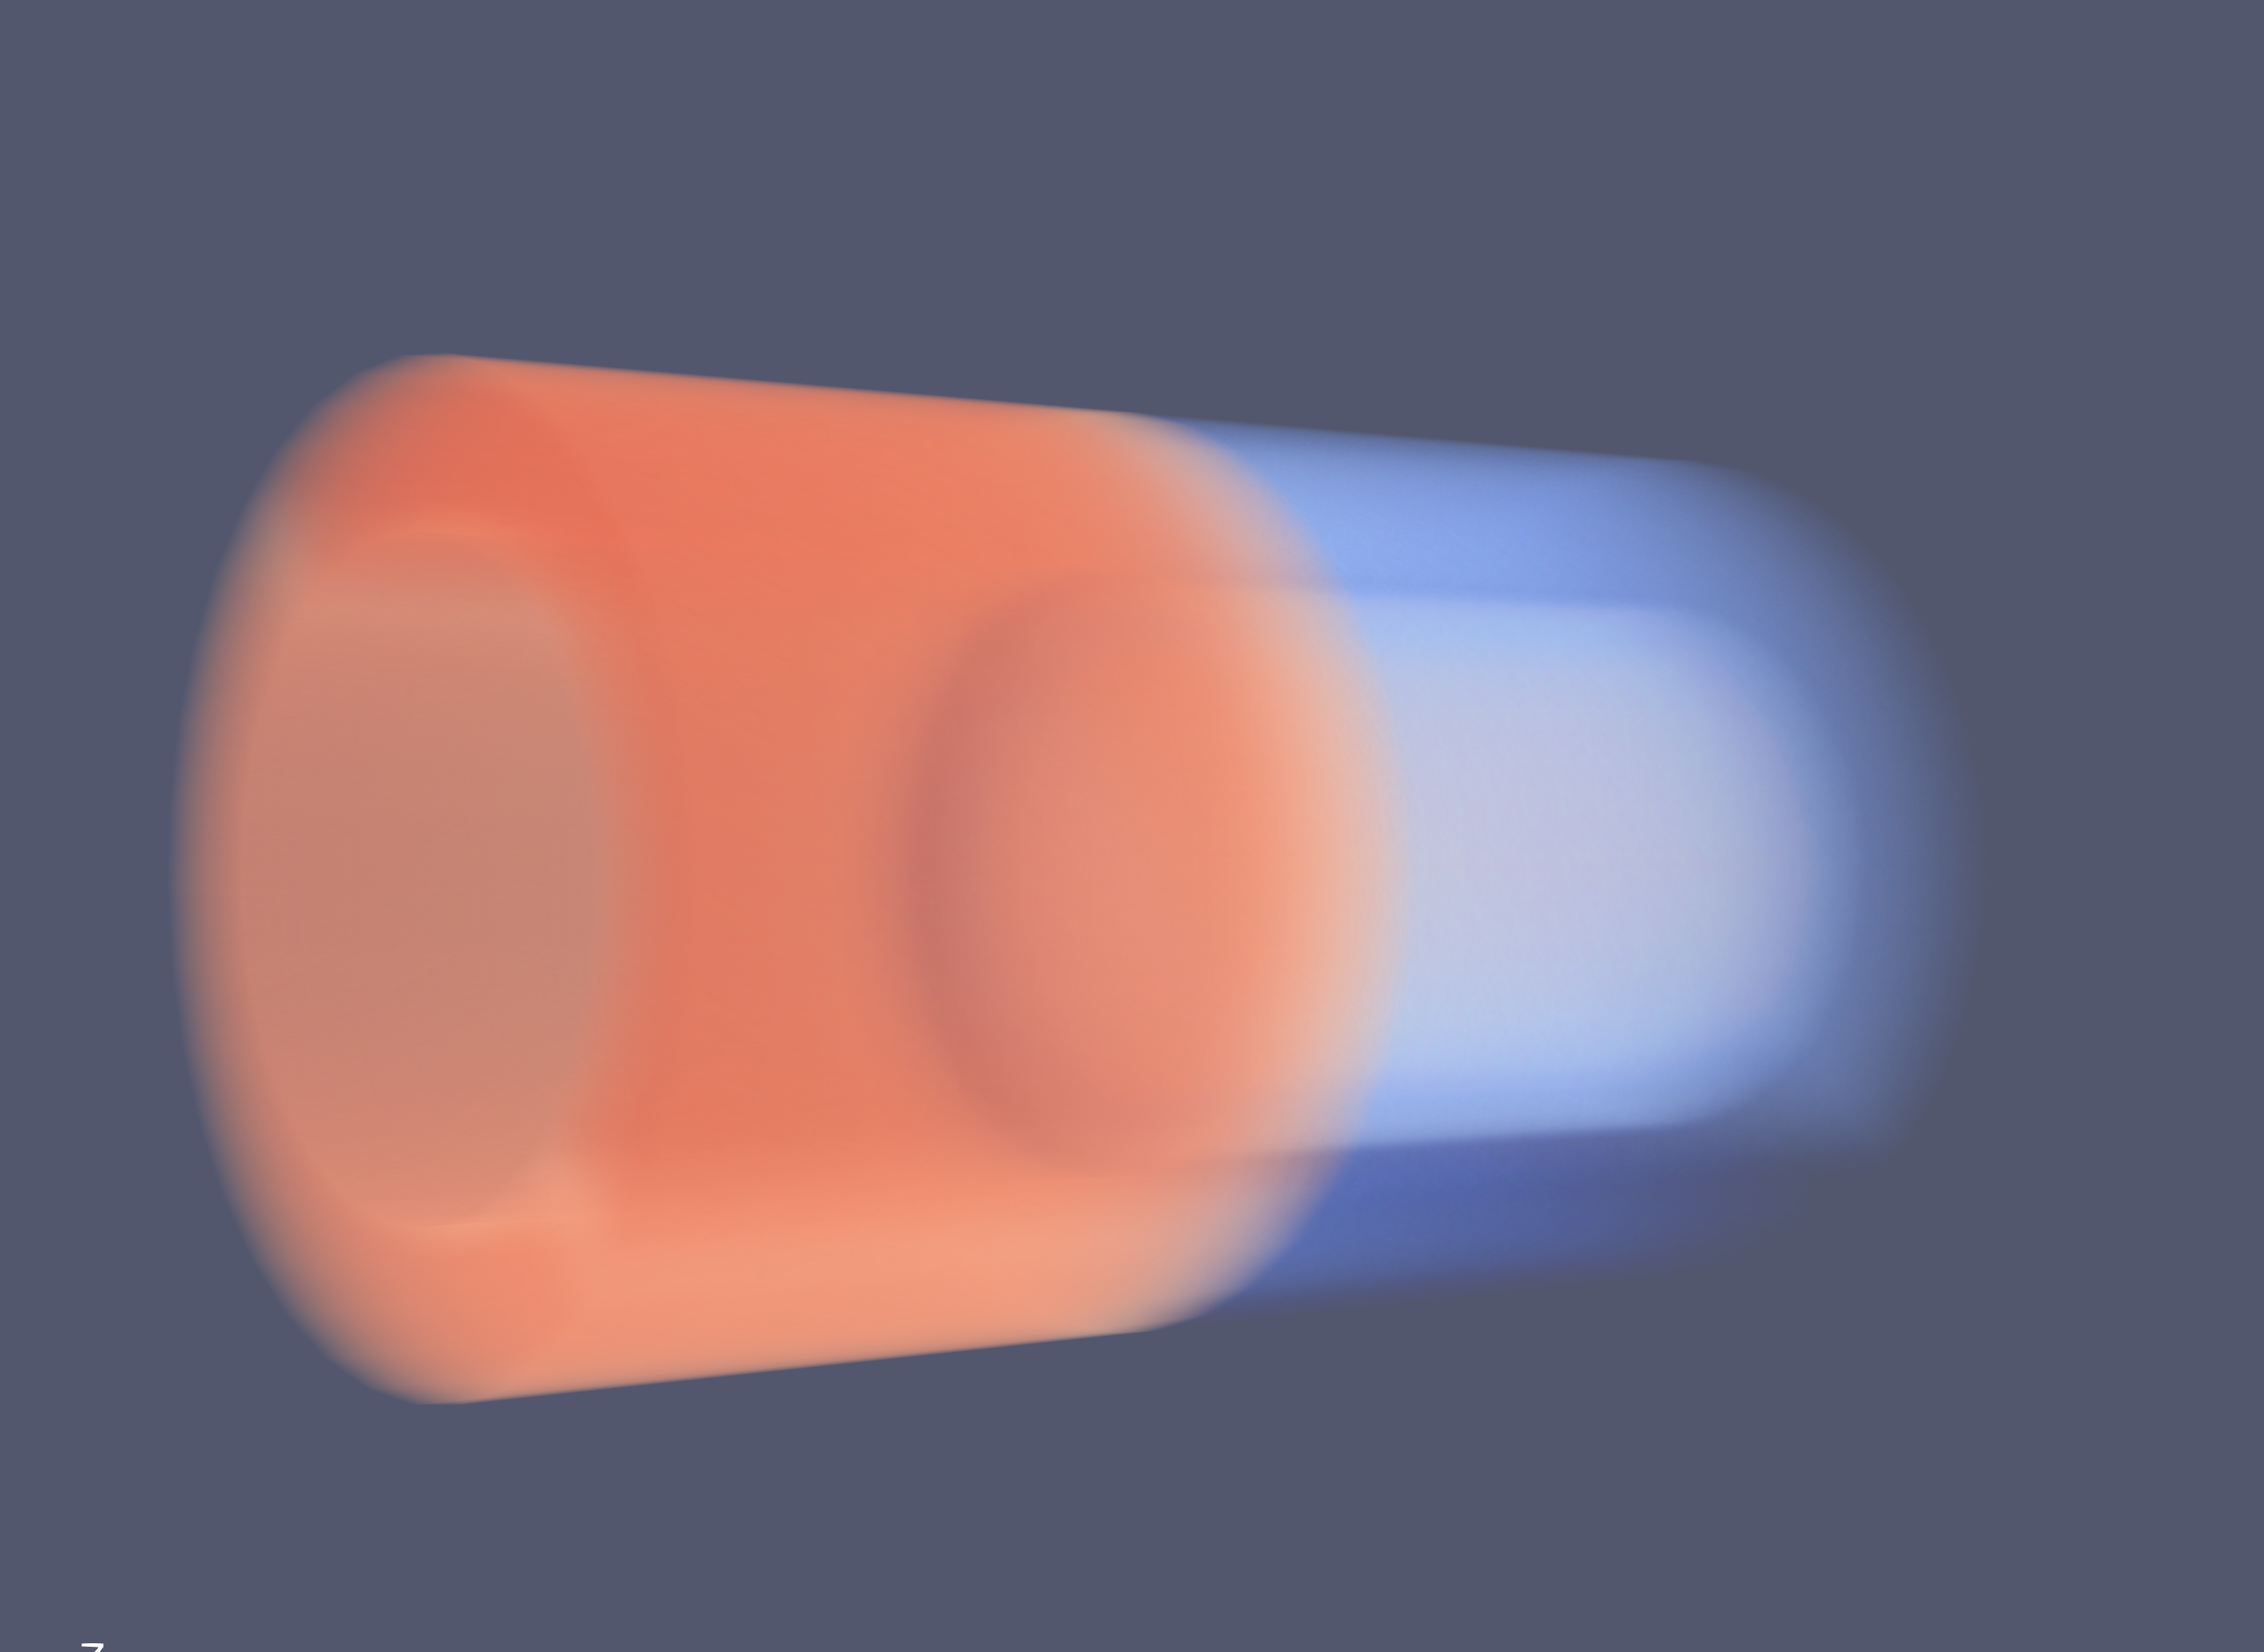
\includegraphics[width=10cm]{Task1.png}
	\item[Tool:]
	\hfill \break
		Paraview.
	\item[Visual Mappings:]
	\begin{itemize}
		\tightlist
		\item[ ]
	\end{itemize}
	\begin{itemize}
		\tightlist
		\item
		\textbf{Mapping 1}: 
		\hfill \break
			The lowest data point 234.336 is set to 0.00 opacity and with a colour blue. The colour blue is then mapped to data point 1462.685 and opacity of 0.592. The third blue data point is at data point 3163.474 and opacity of 0.474.
	\end{itemize}
	
	\begin{itemize}
		\tightlist
		\item
		\textbf{Mapping 2}: 
		\hfill \break
			The red colour mapping starts at data point 5289.462. The first red mapping is at data point 6218.597 with an opacity of 0.828, and the final data point, 10344.588, being mapped deepest red with an opacity of 0.992.
	\end{itemize}
	\begin{itemize}
		\tightlist
		\item
		\textbf{Mapping 3}:
		\hfill \break 
			Colour space used is Diverging and a nan opacity of 1. 
	\end{itemize}
	\item[Data Conversion:] 
	\hfill \break
		Representation of the object is set to Volume. 
	\item[Unique Observation:]
	\hfill \break 
		The visualisation depicts a cylinder, which is half hollow.
	
\end{description}
